% 6 pages max
\documentclass[notitlepage,a4paper,fleqn,9pt]{icmfarticle}
\usepackage[T1]{fontenc}
\usepackage{amsmath}
\usepackage{fancyhdr}
\usepackage{indentfirst}
\usepackage{times}
\usepackage{graphicx}
%\usepackage[dvips]{graphicx}
\usepackage{multicol}
\usepackage{here}
\usepackage[utf8]{inputenc}
\usepackage[T1]{fontenc}
\usepackage[vietnamese,german,english]{babel}

%\usepackage[latin2]{inputenc}

%-----------------------------------------------------------------------------
%\usepackage{psfig}
%\newcommand{\PSFIG}[1]{\psfig{#1}}
%\newcommand{\PSFIG}[1]{}
%-----------------------------------------------------------------------------

\topmargin=-10mm \headsep=5mm \evensidemargin=-12mm
\oddsidemargin=-6mm \textwidth=170mm \textheight=242mm
\columnsep=6mm

\pagestyle{fancy}

\renewcommand{\headrulewidth}{0.1pt}
\fancyhf{} \fancyhead{ \small{\textbf{VIAMC-2017} -- The second Vietnam International Applied Mathematics Conference \hfill October 30th 2017, Hanoi, Vietnam} }
\fancypagestyle{plain}

\setlength{\arrayrulewidth}{0.1pt}
\setlength{\parindent}{0.5cm}
\mathindent0cm

\makeatletter
\renewcommand{\@seccntformat }[1]{\csname the#1\endcsname.\quad}
\renewcommand\section{\@startsection {section}{1}
{-\parindent}{3ex \@plus -1ex \@minus -.2ex}
{3ex \@plus -1ex \@minus -.2ex}{\textbf}}
\renewcommand\subsection{\@startsection {subsection}{2}
{-\parindent}{1.5ex \@plus -1ex \@minus -.2ex}
{1.5ex \@plus -1ex \@minus -.2ex}{\textit}}

\long\def\@makecaption#1#2{%
  \vskip\abovecaptionskip
  \sbox\@tempboxa{#1: #2}%
  \ifdim \wd\@tempboxa >\hsize
    #1: #2\par
  \else
    \global \@minipagefalse
    \hb@xt@\hsize{\box\@tempboxa}%
  \fi
  \vskip\belowcaptionskip}

\renewcommand\maketitle{\par
  \begingroup
    \renewcommand\thefootnote{\@fnsymbol\c@footnote}%
    \def\@makefnmark{\rlap{\@textsuperscript{\normalfont\@thefnmark}}}%
    \long\def\@makefntext##1{\parindent 1em\noindent
%            \hb@xt@1.8em{%
            \hb@xt@0.5em{%
                \hss\@textsuperscript{\normalfont\@thefnmark}}##1}%
    \if@twocolumn
      \ifnum \col@number=\@ne
        \@maketitle
      \else
        \twocolumn[\@maketitle]%
      \fi
    \else
      \newpage
      \global\@topnum\z@   % Prevents figures from going at top of page.
      \@maketitle
    \fi
    \thispagestyle{plain}\@thanks
  \endgroup
  \setcounter{footnote}{0}%
  \global\let\thanks\relax
  \global\let\maketitle\relax
  \global\let\@maketitle\relax
  \global\let\@thanks\@empty
  \global\let\@author\@empty
  \global\let\@date\@empty
  \global\let\@title\@empty
  \global\let\title\relax
  \global\let\author\relax
  \global\let\date\relax
  \global\let\and\relax
}
\makeatother

\renewcommand{\footnoterule}
  {\noindent\rule{\textwidth}{0.1pt}\vspace{1mm}}
\renewcommand{\baselinestretch}{0.913}

\title{\bf 
  Simulation of linear elastic equation and application in mechanics of materials
}
\author{\normalsize\bf
L.Hoang Nguyen, T. Hung Nguyen and T.T. Mai Ta, $^1$
}
\date{\normalsize\vspace{-2ex}\em
$^1$~School of Applied Mathematics and Informatics
Hanoi University of Science and Technology\\
No 1, Dai Co Viet Road, Hanoi, Vietnam\\
\href{mailto:mai.tathitthanh@hust.edu.vn}{mai.tathitthanh@hust.edu.vn},
\href{mailto:tathithanhmai@gmail.com}{tathithanhmai@gmail.com},
\\[1.1mm]
\href{mailto:hoangnl.w@gmail.com}{hoangnl.w@gmail.com},
\href{mailto:hung96ad@gmail.com}{hung96ad@gmail.com}
}
% ---------------------------------------------
% perso : packages and macros
% ---------------------------------------------
\usepackage{latexsym}
\usepackage{mathrsfs}
%\usepackage{amsfonts}
\usepackage{amssymb}
\usepackage{hyperref}
\hypersetup{
colorlinks=true, %colorise les liens
breaklinks=true, %permet le retour a la ligne dans les liens trop longs
urlcolor=blue, %couleur des hyperliens
linkcolor=blue, %couleur des liens internes
citecolor=blue, %couleur des references
pdftitle={An implicit high order discontinuous
	Galerkin level set method
  	for two-phase flow problems}, %informations apparaissant dans
pdfauthor={Ta Pigeonneau Saramito}, %les informations du document
pdfsubject={level set} %sous Acrobat.
}
\newcommand{\Frac}[2] {\displaystyle \frac{#1}{#2}}
\newcommand{\red}[1]  {{\color[rgb]{1,0,0}{{#1}}}}
\renewcommand{\leq}{\leqslant}
\renewcommand{\geq}{\geqslant}
\newcommand{\jump}[1]    {[\![{#1}]\!]}
\newcommand{\average}[1] {\{\!\!\{{#1}\}\!\!\}}
% ---------------------------------------------
\begin{document}

\raggedcolumns

\maketitle
\vspace{-3mm}
\noindent\rule{\textwidth}{.1pt}

\noindent
Abstract\\
\vspace{1ex}

\noindent
A numerical method for linear elastic equation is presented and its application in mechanics of materials is investigated in two and three dimensions. The programs are written in FreeFem++, a free environment to solve a variety of Partial Differential Equations using the Finite Element method. The results of numerical tests are compared with the studies in Mechanical engineering showing the applicability of present software in solving class of technical problems. \\

\vspace{1ex}

\noindent {\em Keywords: Linear elastic equation, continuous Galerkin FEM}

% ligne de separation
\noindent\rule{\textwidth}{.1pt}\vspace{2mm}

\begin{multicols}{2}
% --------------------------------------------------------------------
\section{Introduction}
\label{sec:introduction}
% --------------------------------------------------------------------
Elasticity interface problems have wide applications in strength of materials, also called mechanics of materials or in continuum mechanics, particularly for problems that involve stresses and strains, see for example \cite{Yu86,FS96}. In mechanics of materials, the strength of a material is its ability to withstand an applied load without failure or plastic deformation. The field of strength of materials deals with forces and deformations that result from their acting on a material.

In this paper, we propose a finite element method for plane elasticity problems in which the physical parameters and solutions may be discontinuous across an arbitrary interface. This work is motivated by the locally modified triangulations proposed in \cite{Bor90, XILT08} for Poisson equations on irregular domains. The non-conforming finite element method proposed in \cite{LLW03} is simple and enforces the homogeneous jump condition but it is not fully second order accurate because the basis functions are non-conforming. The conforming finite element method proposed in \cite{GLL08, LLW03} is second order accurate but it is not easy to implement as the basis functions have wider support in the neighborhood of the interface. 
We refer the reader to \cite{TG85,Sad05} for more information of the elasticity problems.
In the present scheme, we want to take advantage of FreeFem using triangular meshes \url{http://www.freefem.org}. The main contribution is that we use such regular triangulation meshes to solve the elasticity problem with interfaces using the continuous Galerkin finite element method. Numerical experiments in model examples in computational mechanics illustrate the efficient and reliability of present work.

The paper is organized into five sections. Section~\ref{sec:model} provides a brief description of our model problem. Section \ref{sec:method} presents the weak formulation and finite element discretization. The numerical results are presented in section~\ref{sec:result}. Section~\ref{sec:conclusion} gives some comments and perspectives for the present work.
% -------------------------------------------------------------------
\section{Setting of the problem} 
\label{sec:model}
Let us introduce the problem of our interest: consider an elastic plate which occupies, in its reference configuration, a bounded domain $\Omega \subset \mathbb{R}^d$ ($d$ = 2 or 3) with a boundary $\Gamma = \{\Gamma_D, \Gamma_N\}$. We assume Dirichlet conditions on $\Gamma_D$ and Neumann conditions on $\Gamma_N$. 
Let $u$ be the displacement of a plate which is composed of different materials. The relation between strain tensor and displacements of the plate is given by:
$$e(u) = (\nabla u + \nabla u^t)/2$$
Assuming that the material is linearly elastic and isotropic; and that the displacements are small, Hooke's law gives a relationship between the stress tensor and the strain tensor :
$$\mathcal{A}e(u) = 2\mu e(u) + \lambda Tr(e(u))Id$$
where $\mathcal{A}e(u)$ is the stress tensor, $Id$ the identity matrix, $Tr(.)$ the trace function and $\mu$, $\lambda$ are the Lam'e coefficients that describe the mechanical properties of the solid, and are themselves related to the better known constants $E$, Young's modulus, and $v$, Poisson's ratio:
$$\mu = \frac{E}{2(1 + v)}, \qquad \lambda = \frac{Ev}{(1 + v)(1 - 2v)}.$$
We denote by $f$ the vector-valued function of the volume forces and by $g$ that of the surface loads. The displacement field $u$ in $\Omega$ is the solution of the linearized elasticity system (\ref{prob})
\begin{equation}\label{prob}
\quad\quad\quad\quad\quad
\begin{cases}
-\text{div}(\mathcal{A}e(u)) = f \qquad \text{in } \Omega,\\
u = 0 \quad\qquad\qquad\qquad \text{on } \Gamma_D, \\
\mathcal{A}e(u))n = g \qquad\qquad \text{on } \Gamma_N.
\end{cases}
\end{equation}

\section{Numerical method}
\label{sec:method}
%---------------------------------------------
\subsection{Variational formulation}
The numerical resolution of this problem by a finite element method evidently involves a variational formulation. Let $v \in (H^1(\Omega))^2$ be a test function, the corresponding variationnal form is:
$$-\int_\Omega\text{div}(\mathcal{A}e(u)).v = \int_\Omega f.v$$
We use the Green's theorem as:
$$\int_\Omega\mathcal{A}e(u).\nabla v = \int_\Omega f.v + \int_{\partial \Omega}(\mathcal{A}e(u)n).v$$
Choose the test function $v = 0|\Gamma_D$, we have:
$$\int_\Omega\mathcal{A}e(u):e(v) = \int_\Omega f.v + \int_{\Gamma_N}g.v$$
where : denote the tensor scalar product, i.e. $a : b = \sum_{ij}{a_{ij}b_{ij}}.$ \\
So the variationnal form can be written by the following form:
$$\int_\Omega 2\mu e(u) : e(v) + \lambda(\text{div}u)(\text{div}v) = \int_\Omega f.v + \int_{\Gamma_N}g.v.$$
According the Lax-Milgram lemma, there exists a weak solution of (\ref{prob}) for reasonable boundary conditions \cite{LAX-1994, LAX-1987}.
% --------------------------------------------
\subsection{Finite element discretization}
% --------------------------------------------
For the implementation, problem (1) is discretized using the finite element
method. The space $V$ is replaced by the finite dimensional subspace $V_N$. The discretized problem (P): Find $u_h \in V_N$
such that $u_h = 0$ on $\Gamma_D$ and, for all $v_h \in V_N$ with $v_h = 0$ on $\Gamma_D$,
$$\int_\Omega 2\mu e(u_h) : e(v_h) + \lambda(\text{div}u_h)(\text{div}v_h) = \int_\Omega f.v_h + \int_{\Gamma_N}g.v_h$$
Let $\mathcal{T}$ denote a triangulation of $\Omega$ and let $\mathcal{N}$ be the set of the all nodes in $\mathcal{T}$; set $(\eta_k,...,\eta_{dN})=(\varphi_1e_1, \varphi_2e_2,...,\varphi_1e_d,...,\varphi_Ne_1,\varphi_Ne_2,...,\varphi_Ne_d)$ be the nodal basic of the finite dimensional space $V_N$, where $N$ is the number of nodes of the mesh, $d$ the dimension of the displacement vector, and $\varphi_i$ is the scalar hat function of node $x_i$ in the triangulation $\mathcal{T}$:
$$\varphi_{x_i}(x_j) = \begin{cases}
1 \text{ with } x_i = x_j, \\
0 \text{ with } x_i \neq x_j.
\end{cases}$$
Apply to boundary conditions with $i = 1,...,dN$:
$$\int_\Omega 2\mu e(u_h) : e(\eta_i) + \lambda(\text{div}u_h)(\text{div}\eta_i) = \int_\Omega f.\eta_i + \int_{\Gamma_N}g.\eta_i.$$
For the discrete displacement vector we have $u_h = \sum_{j=1}^{dN}U_i\eta_i$ and the flowing below is the linear system of equations:
$$\displaystyle\sum^{dN}_{i=1}(\displaystyle\int_\Omega 2\mu e(\eta_j) : e(\eta_i) + \lambda(\text{div}\eta_j)(\text{div}\eta_i)) = \int_\Omega f.\eta_i + \int_{\Gamma_N}g.\eta_i.$$
The stiffness matrix $A=(A_{ij})\in\mathbb{R}^{dN x dN}$ and the right hand side $b=(b_i)\in\mathbb{R}^{dN}$ are defined as
$$A_{ij}=\displaystyle\int_\Omega 2\mu e(\eta_j) : e(\eta_i) + \lambda(\text{div}\eta_j)(\text{div}\eta_i),$$
$$b_i=\int_\Omega f.\eta_i + \int_{\Gamma_N}g.\eta_i.$$
The stiffness matrix is sparse, symmetric and positive semi-definite. The condition $u_h = 0$ on $\Gamma_D$ and $v_h = 0$ on $\Gamma_D$ will be incorporated.
%----------------------------------------------------------------------

%----------------------------------------------------------------------
\section{Numerical experiments}
\label{sec:result}
Many parameters and measurements in the physical sciences and engineering are expressed as a concrete number - a numerical quantity and a corresponding dimensional unit. Often a quantity is expressed in terms of several other quantities; for example, gravitational acceleration is a combination of length and time, e.g. 9.81 metres per second squared. Compound relations with "per" are expressed with division, e.g. 9.81m / 1$s^2$. Sometimes the names of units obscure that they are derived units. For example, one newton is 1 $kg.m/s^2$. The seven base quantities and their corresponding units are: length (metre-m), mass (kilogram-kg), time (second-s), electric current (ampere-A), thermodynamic temperature (Kelvin-K), amount of substance (mole-mol), luminous intensity (candela-cd). \\
In elasticity, it is usual to display undeformed and deformed meshes. In the graphical representation of the deformed mesh, a magnification factor is used for the displacement. In all examples, we convert all physical quantity to the same units as the table below and remove physical quantity.

\begin{center}
\begin{tabular}{ |c|c|c| } 
 \hline
 Measure & Symbol & Unit \\ 
 \hline
 Length or radius & $r_i, r_e, x, y$ & $mm, m$ \\ 
 Young's modulus & $E$ & $N/mm^2, N/m^2$ \\ 
 Gravity Force & $g$ & $N$ \\ 
 Forces & $F$ & $N$ \\ 
 External forces & $f$ & $N/mm, N/m$ \\ 
 Pressure & $p$ & $N/mm^2, N/m^2$ \\ 
 \hline
\end{tabular}
\end{center}

\subsection{Membrane}
A membrane is clamped at $x=0$ and subjected to a volume force $f=(0,1)$ at $x=35$ and shearing load $g=(0,-0.981)$ with Young's modulus and Poisson's ratio $E=3e4, v=0,4$ \cite{Koko-2007}.
\begin{figure}[H]
  \begin{center}
    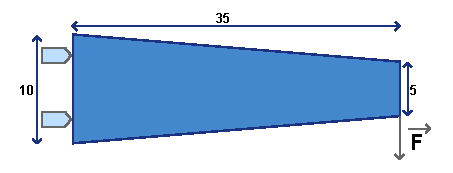
\includegraphics[width=0.4\textwidth]{4-1.pdf}
  \end{center}
  \caption{The membrane: initial configuration.}
  \label{exam11}
\end{figure}
Figures \eqref{exam12} below show initial configuration and deformed configurations of the membrane, for a mesh with 1606 triangles:
\begin{figure}[H]
  \begin{center}
    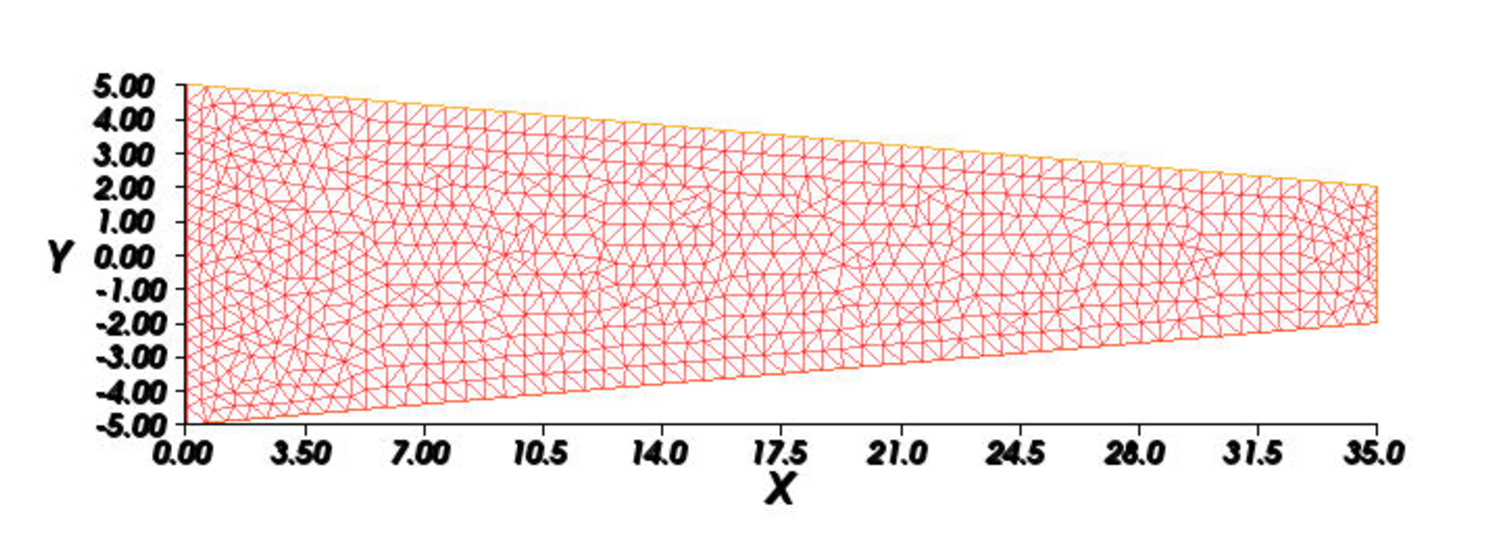
\includegraphics[width=0.4\textwidth]{4-1-1.pdf}
  \end{center}
  \caption{The membrane: initial configuration mesh.}
  \label{exam12}
\end{figure}
The magnification factor, for the displacement field, is 20. So, we have deformed mesh for membrane in the figure \eqref{exam13} .
\begin{figure}[H]
  \begin{center}
    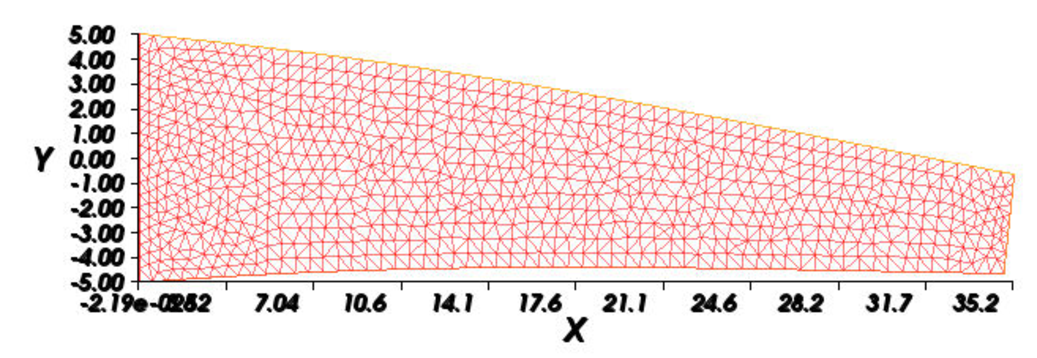
\includegraphics[width=0.4\textwidth]{4-1-2.pdf}
  \end{center}
  \caption{Deformed mesh for membrane.}
  \label{exam13}
\end{figure}



\subsection{Traction force}
A metal plate with a hole in its center (figure 4) is subjected to a traction force with $F=[0,1e4]$ at $x=0.4$ and shearing load $g=(0,-9.81)$ with Young's modulus and Poisson's ratio $E=7e4, v=0,3$ \cite{TIT-07}. The initial mesh with 1607 triangles like figure \eqref{exam21}.
\begin{figure}[H]
  \begin{center}
    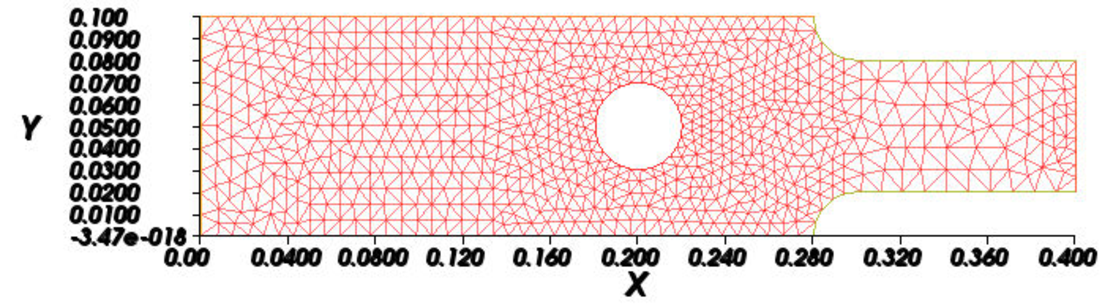
\includegraphics[width=0.4\textwidth]{4-2-1.pdf}
  \end{center}
  \caption{The metal plate: initial configuration.}
  \label{exam21}
\end{figure}
The figure \eqref{exam22} show deformed configurations of metal plate being subjected to a traction force F=100. Because the forces is small and localised, the deformation isn't large.
\begin{figure}[H]
  \begin{center}
    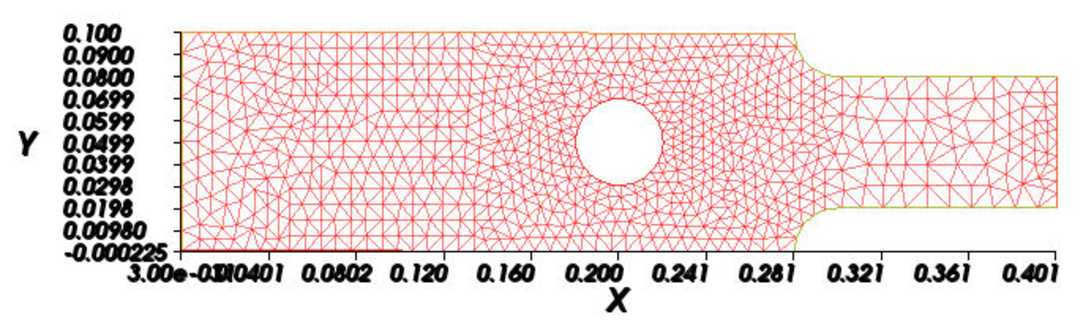
\includegraphics[width=0.4\textwidth]{4-2-2.pdf}
  \end{center}
  \caption{The metal plate: deformed configuration with F=100.}
  \label{exam22}
\end{figure}
But with F=5e3 (figure \eqref{exam23}) and F=1e4 (figure \eqref{exam24}), the deformation is large. The blue tones visualize the approximate Von Mises effective stress.
\begin{figure}[H]
  \begin{center}
    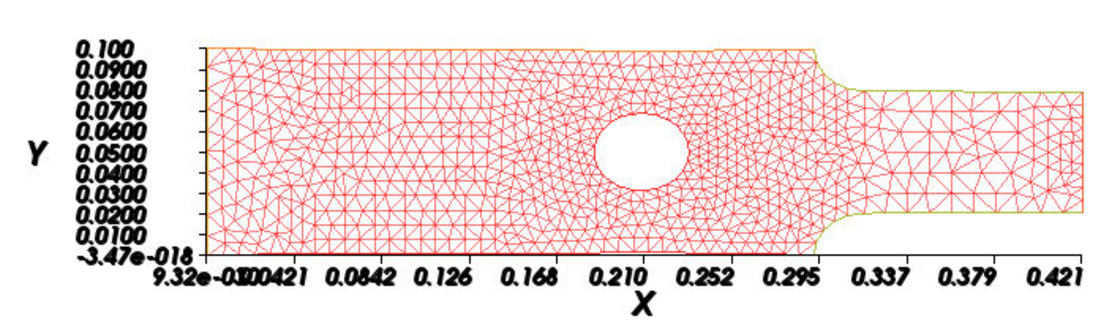
\includegraphics[width=0.4\textwidth]{4-2-3.pdf}
  \end{center}
  \caption{The metal plate: deformed configuration with F=5e3.}
  \label{exam23}
\end{figure}
\begin{figure}[H]
  \begin{center}
    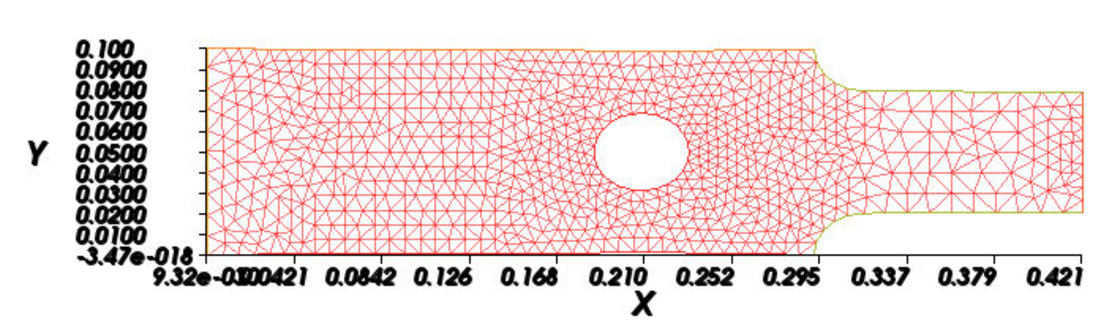
\includegraphics[width=0.4\textwidth]{4-2-3.pdf}
  \end{center}
  \caption{The metal plate: deformed configuration with F=1e4.}
  \label{exam24}
\end{figure}
\subsection{Compression force}
Another metal plate with a hole in its center is subjected to a compression force with $f=(-1e4,0)$ and shearing load $g=(0,-9.81)$ with Young's modulus and Poisson's ratio $E=7e4, v=0,3$ \cite{TIT-07}. Similar, we have figure \eqref{exam31} - initial mesh and figure \eqref{exam32} - deformed mesh configurations of metal plate being impacted by compression force.
\begin{figure}[H]
  \begin{center}
    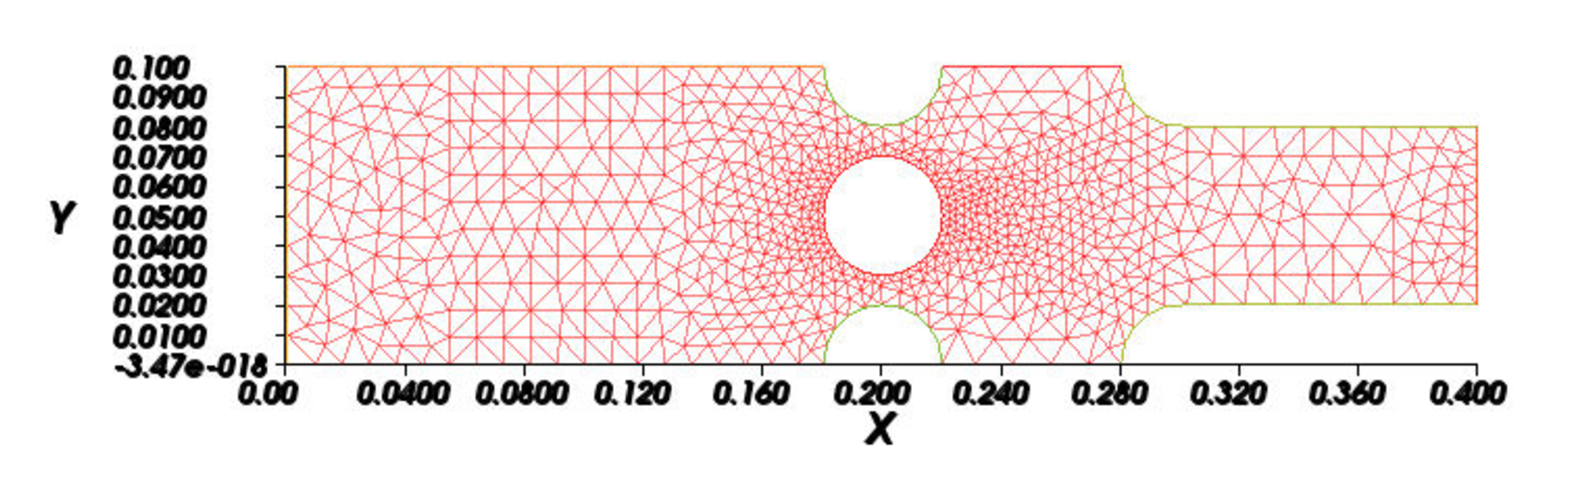
\includegraphics[width=0.4\textwidth]{4-3-1.pdf}
  \end{center}
  \caption{The metal plate: initial configuration.}
  \label{exam31}
\end{figure}
\begin{figure}[H]
  \begin{center}
    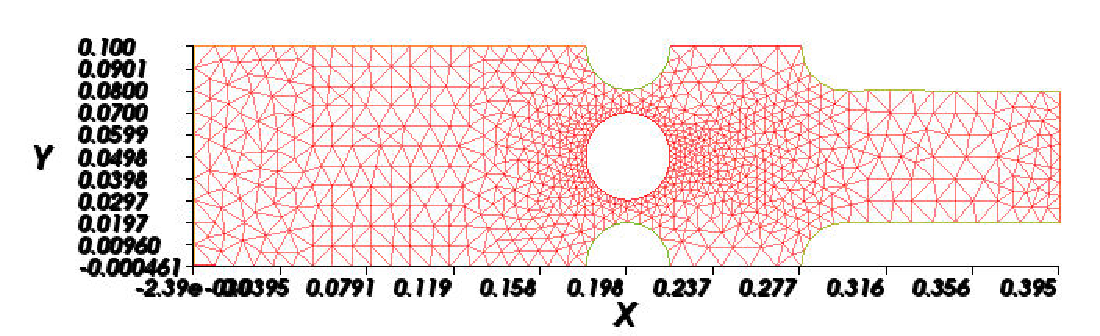
\includegraphics[width=0.4\textwidth]{4-3-2.pdf}
  \end{center}
  \caption{The metal plate: deformed configuration.}
  \label{exam32}
\end{figure}

We consider a plate consist of two materials with a non-circle interface in a state of plane strain. The interface is given by $r = 0.5 + 0.2 sin(kt)$ in polar coordinates. In this example, we set $k=5$. The plate is $2 * 2$ with the bottom fixed and $f = 1e7$ force applied on the top. The Young's modulus and Poisson's ratio for the inner and outer materials are $E=1e9, v=0,3$ \cite{HUI-2011}. The initial mesh with 5796 triangles like figure \ref{exam33} below:

\begin{figure}[H]
  \begin{center}
    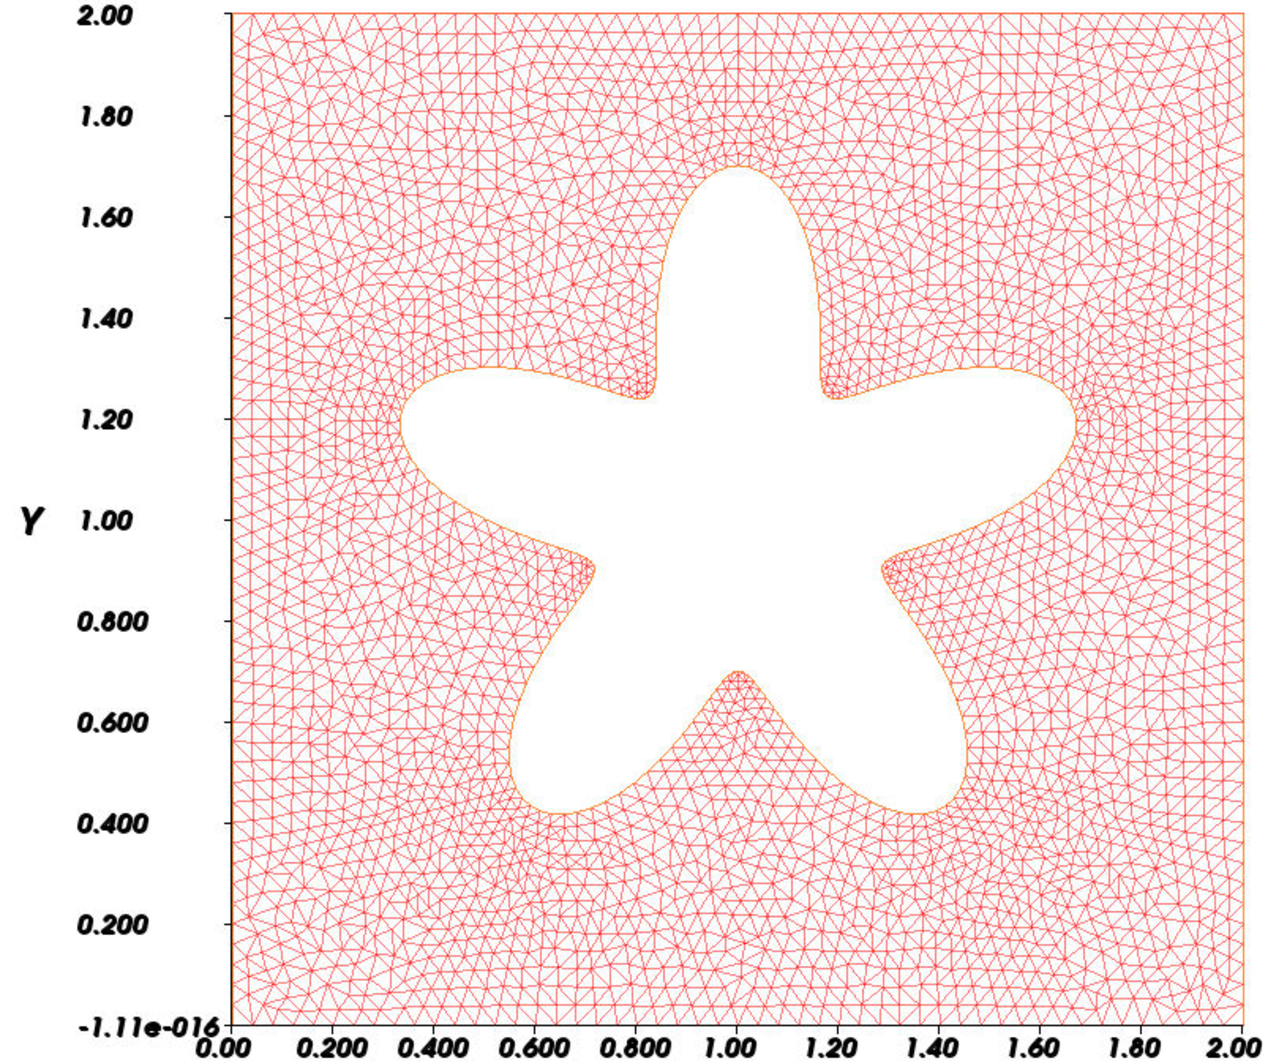
\includegraphics[width=0.4\textwidth]{4-3-3.pdf}
  \end{center}
  \caption{A rectangular plate with a non-circle interface $r = 0.5 + 0.2sin(5t)$.}
  \label{exam33}
\end{figure}

Under the pressure, the plate will undergo a compression in y-direction and will react by stretching in the x-direction in order to reduce the change in the volume.\\
We show the contour plot for the displacement distribution.

\begin{figure}[H]
  \begin{center}
    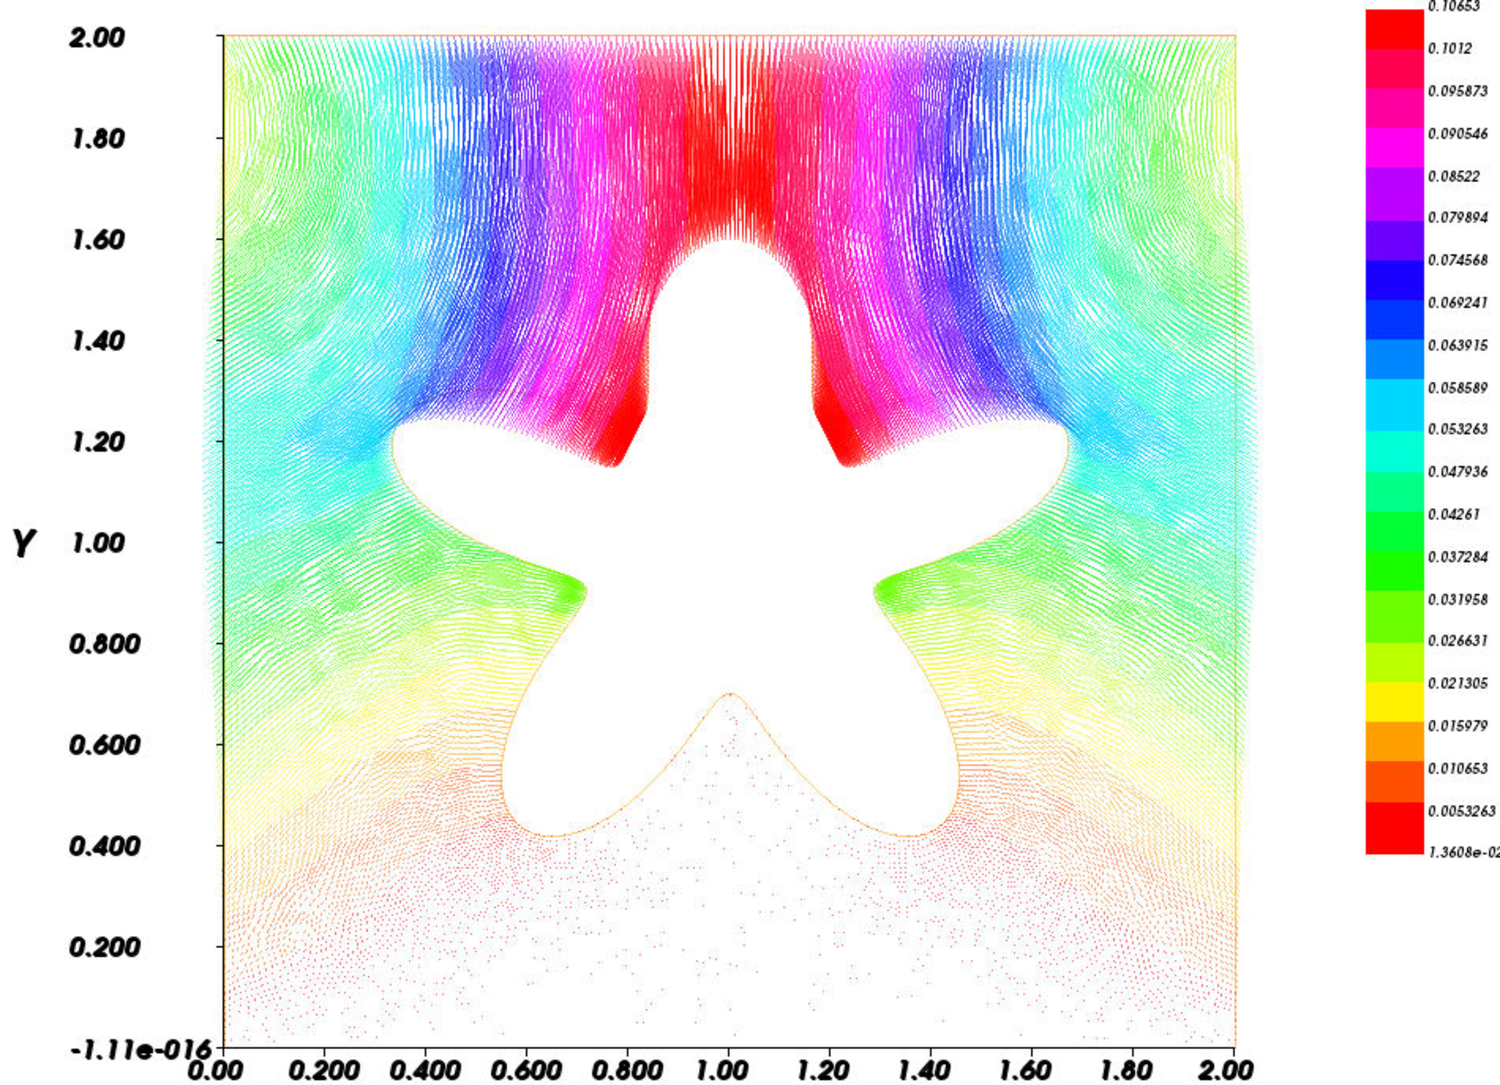
\includegraphics[width=0.4\textwidth]{4-3-4.pdf}
  \end{center}
  \caption{Displacement distribution of the plate.}
  \label{exam34}
\end{figure}

Figure \ref{exam35} the position of the deformed plate.

\begin{figure}[H]
  \begin{center}
    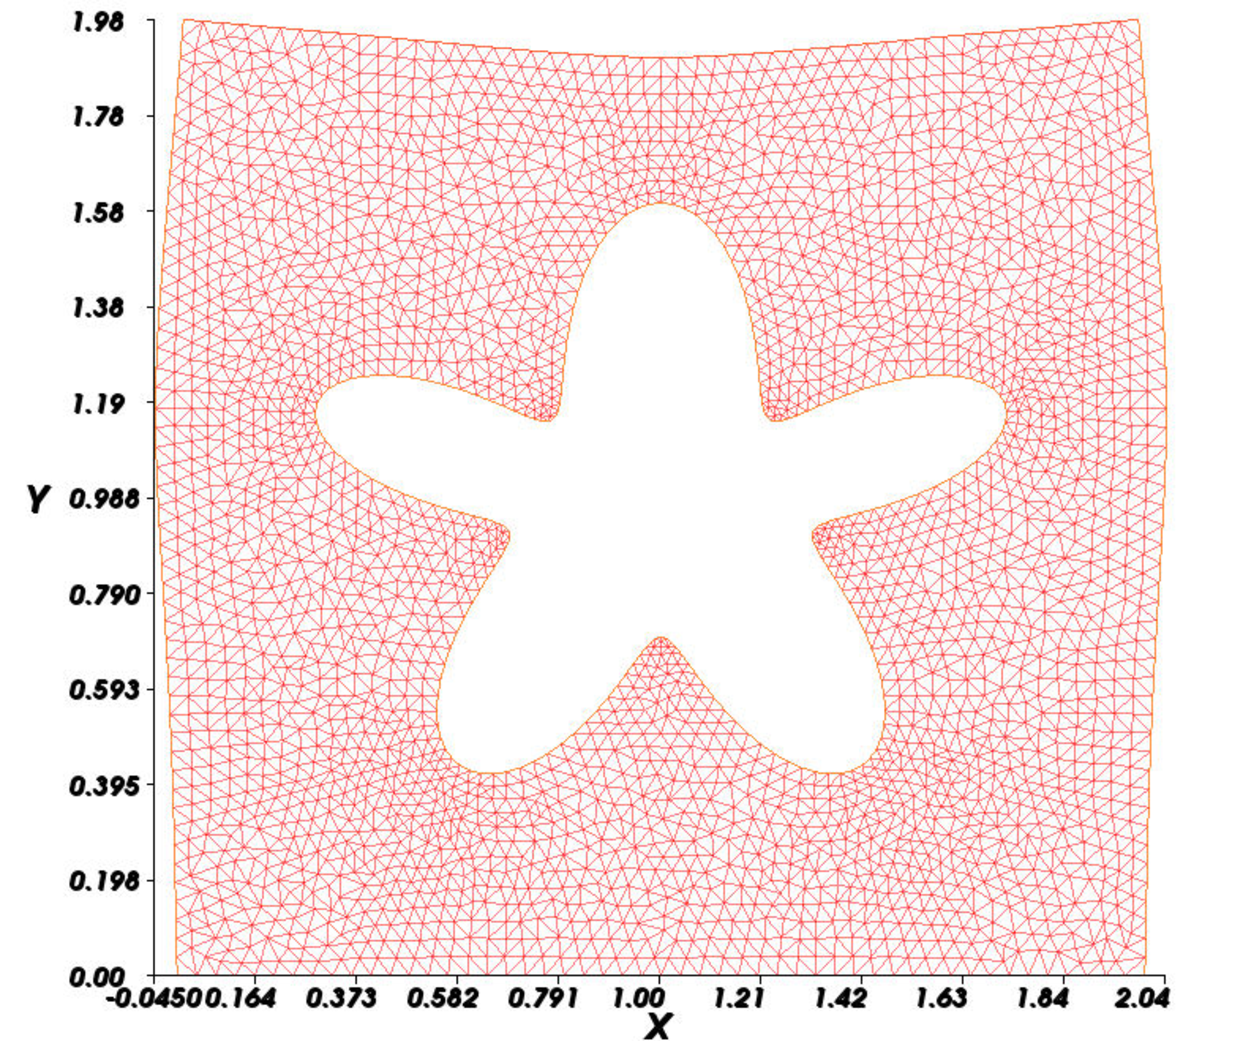
\includegraphics[width=0.4\textwidth]{4-3-5.pdf}
  \end{center}
  \caption{Deformed plate.}
  \label{exam35}
\end{figure}

\subsection{Internal pressure}
An annular metal is subjected to internal pressure as figure \eqref{exam41} with $p=1e3,E=2e5, v=0.3, r_i=42, r_e=50, h=1 (h<<r_i)$ \cite{TIT-07}. Because of $(h<<r_i)$, do it just a two-dimensional problem. In the next example, we consider a metal tube with the same $p, E, v, r_i, r_e$ but have the length of metal tube $h$. The problem become a three-dimensional problem.
\begin{figure}[H]
  \begin{center}
    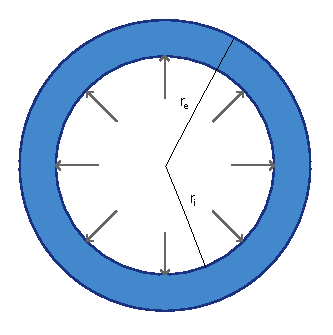
\includegraphics[width=0.3\textwidth]{4-4.pdf}
  \end{center}
  \caption{The annular metal is affected by internal pressure.}
  \label{exam41}
\end{figure}
The initial mesh with 1144 triangles:
\begin{figure}[H]
  \begin{center}
    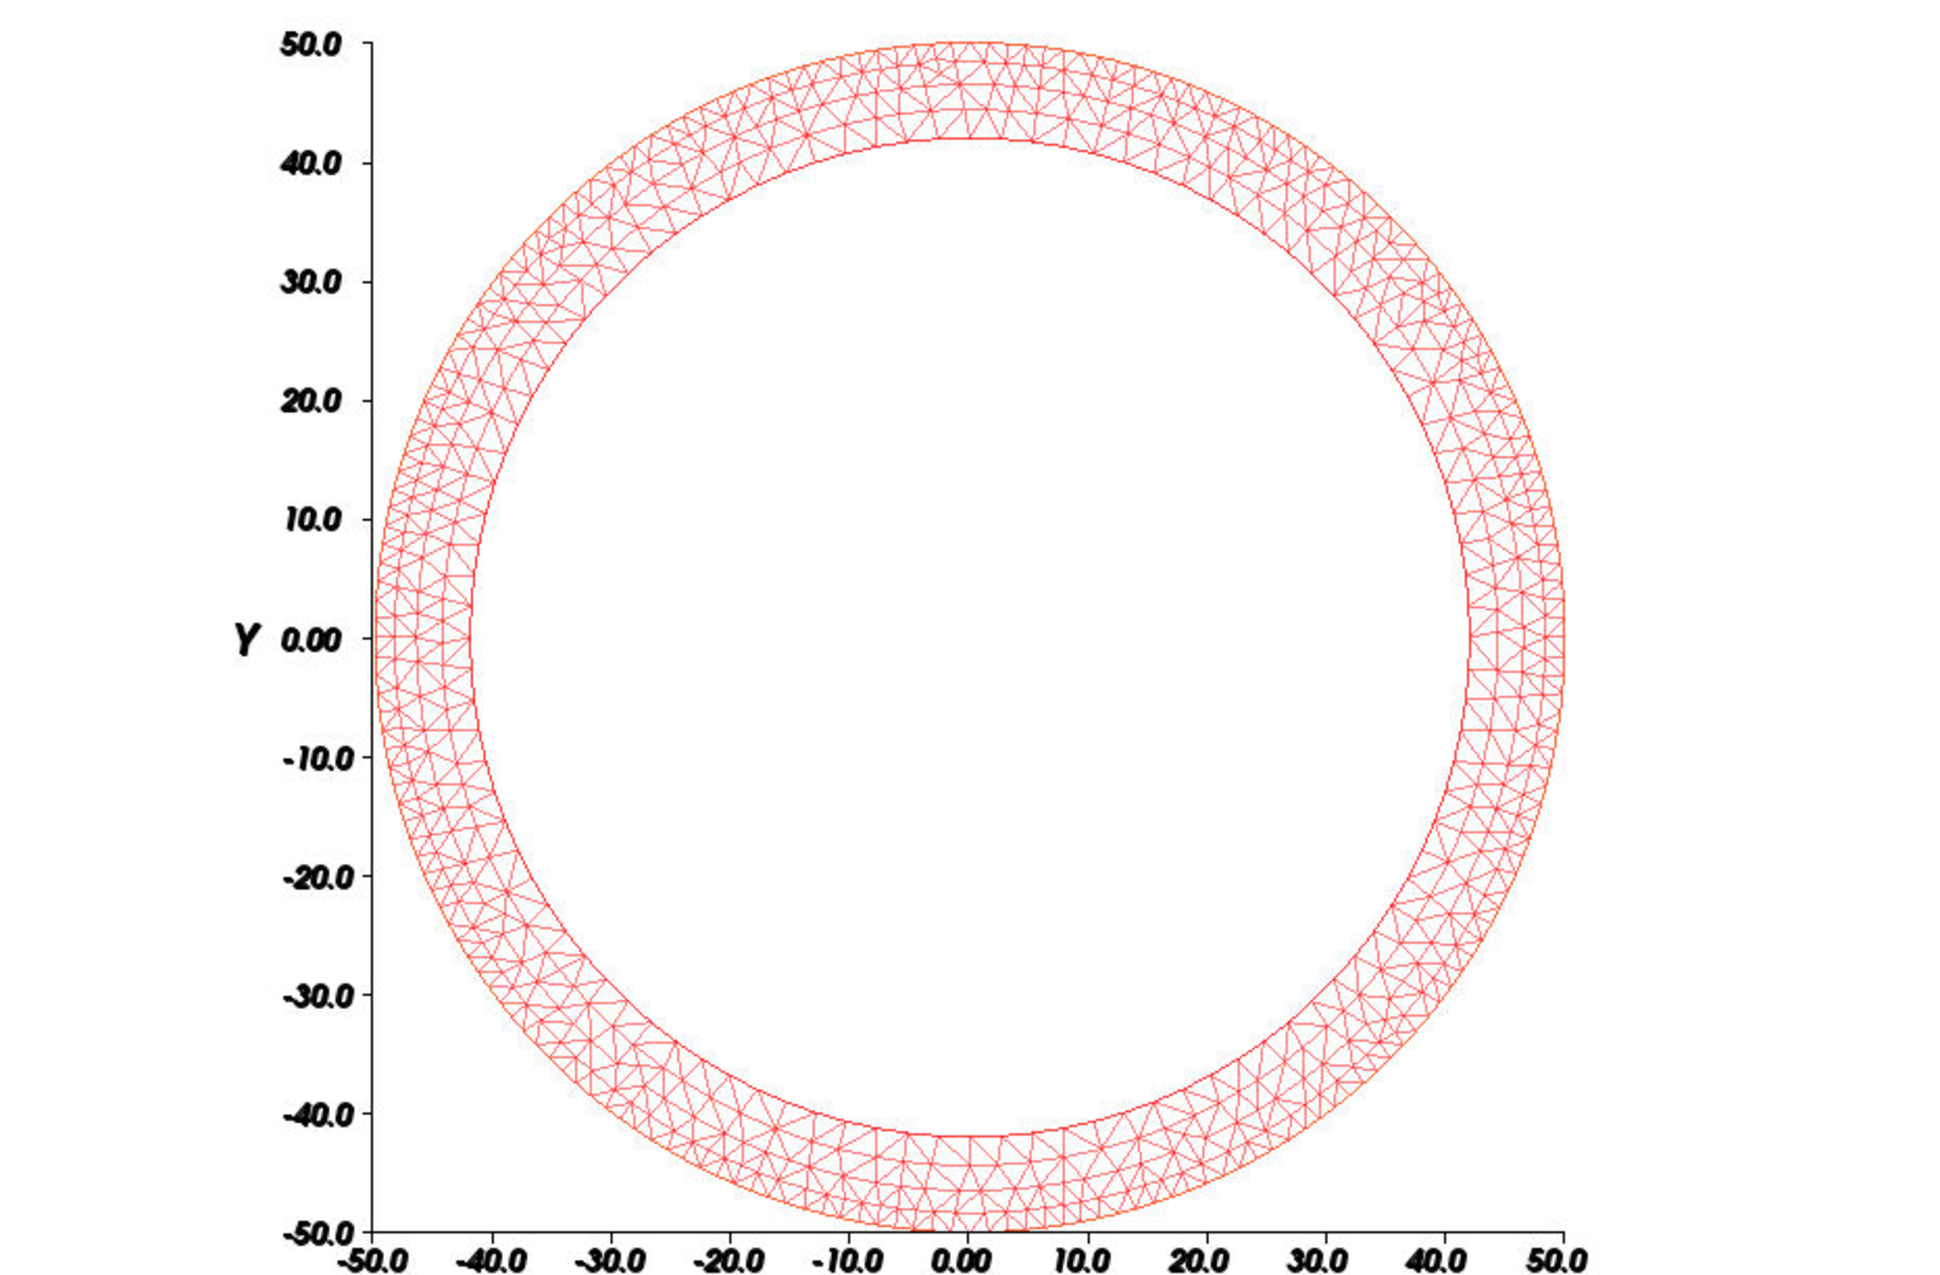
\includegraphics[width=0.4\textwidth]{4-4-1.pdf}
  \end{center}
  \caption{The annular is subjected to internal pressure.}
  \label{exam42}
\end{figure}
Figure \eqref{exam43} shows deformed configurations of the annular when subjected to internal pressure:
\begin{figure}[H]
  \begin{center}
    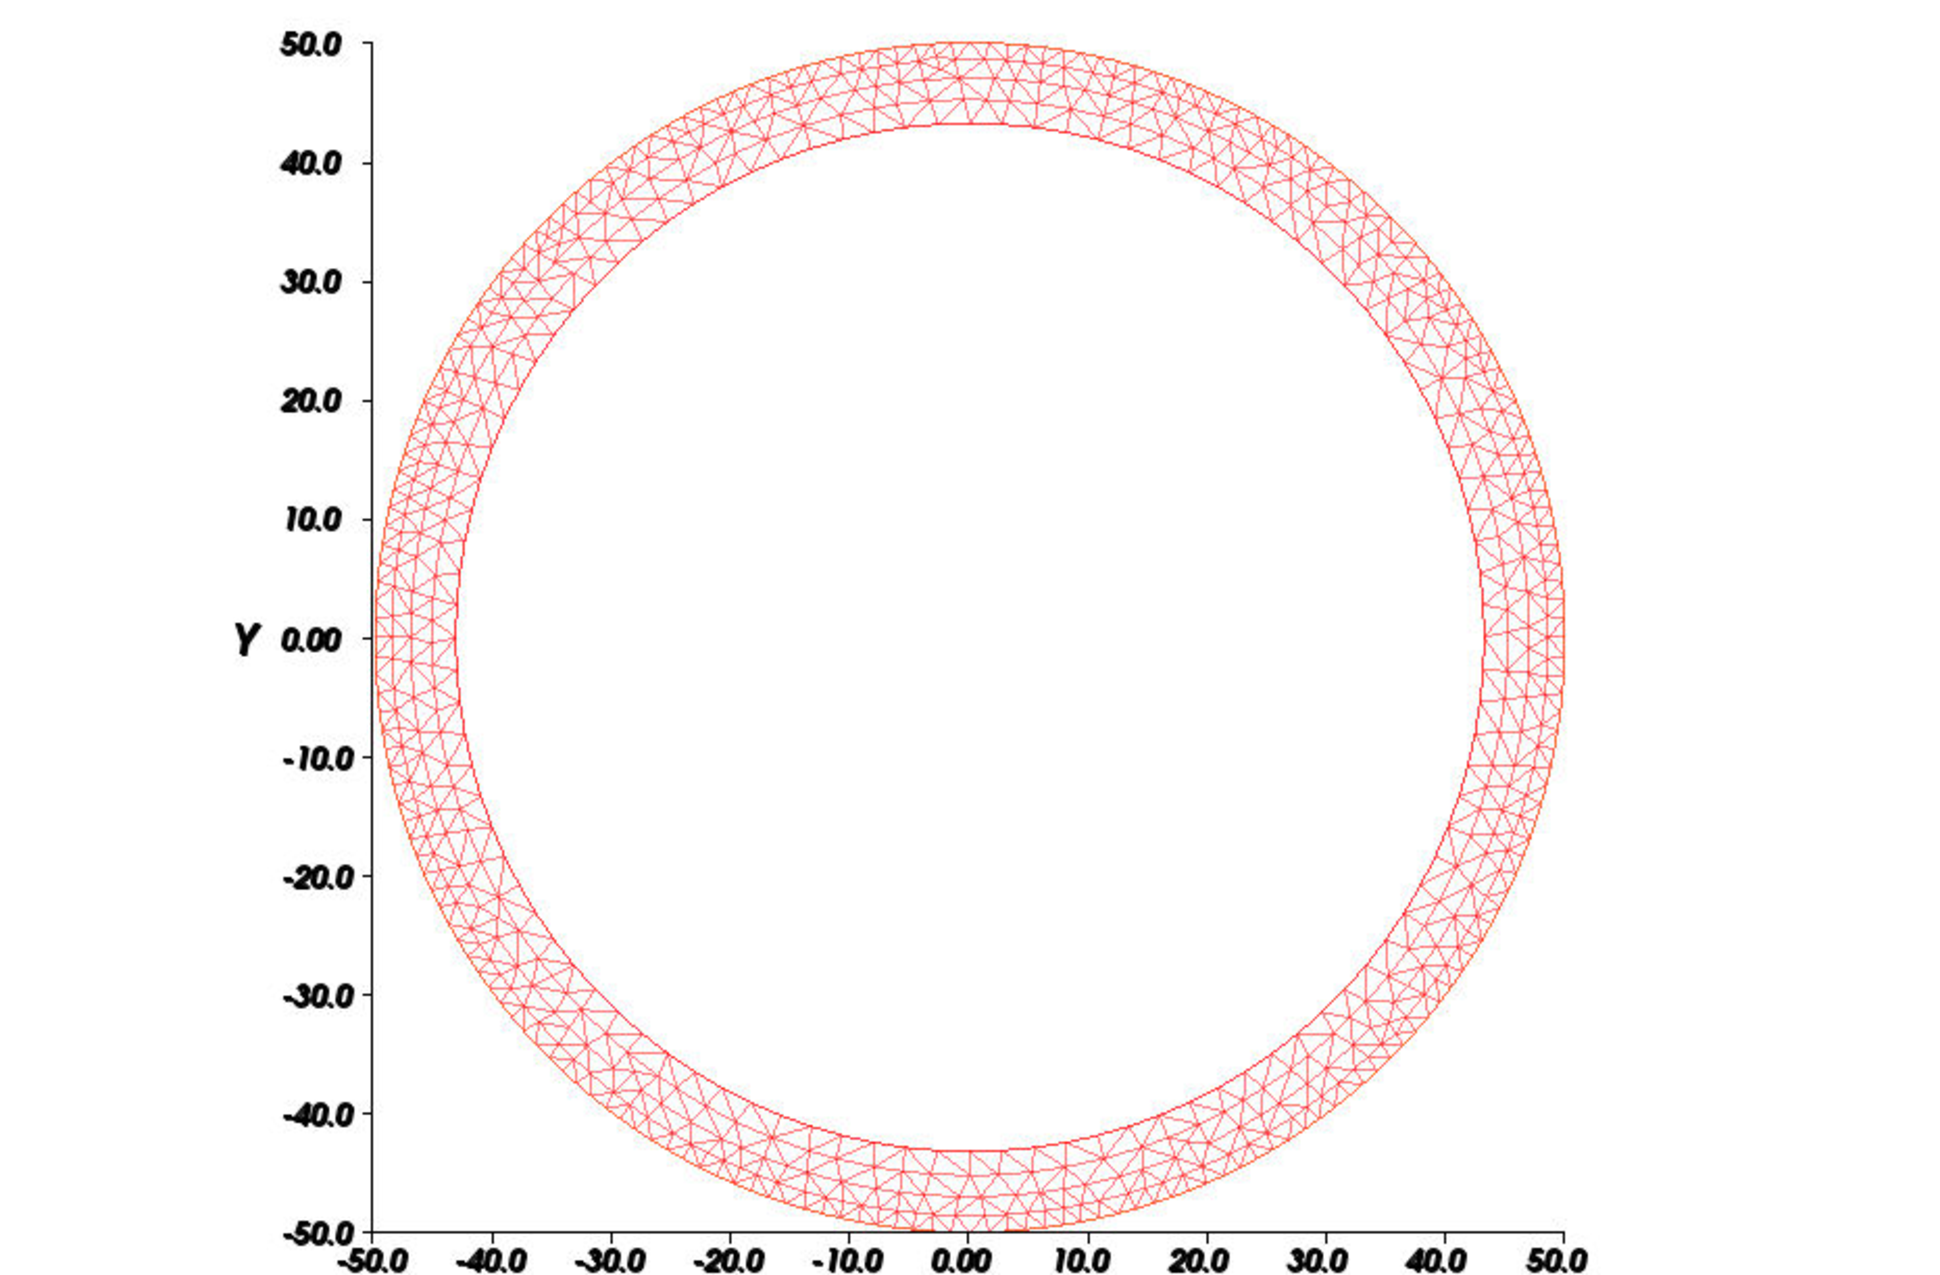
\includegraphics[width=0.4\textwidth]{4-4-2.pdf}
  \end{center}
  \caption{The annular: deformed configuration.}
  \label{exam43}
\end{figure}

As in above, we consider a metal tube. Which is subjected to internal pressure as figure 8 with $p=1e3,E=2e5, v=0.3, r_i=40, r_e=50$ and the length $h=40$.
\begin{figure}[H]
  \begin{center}
    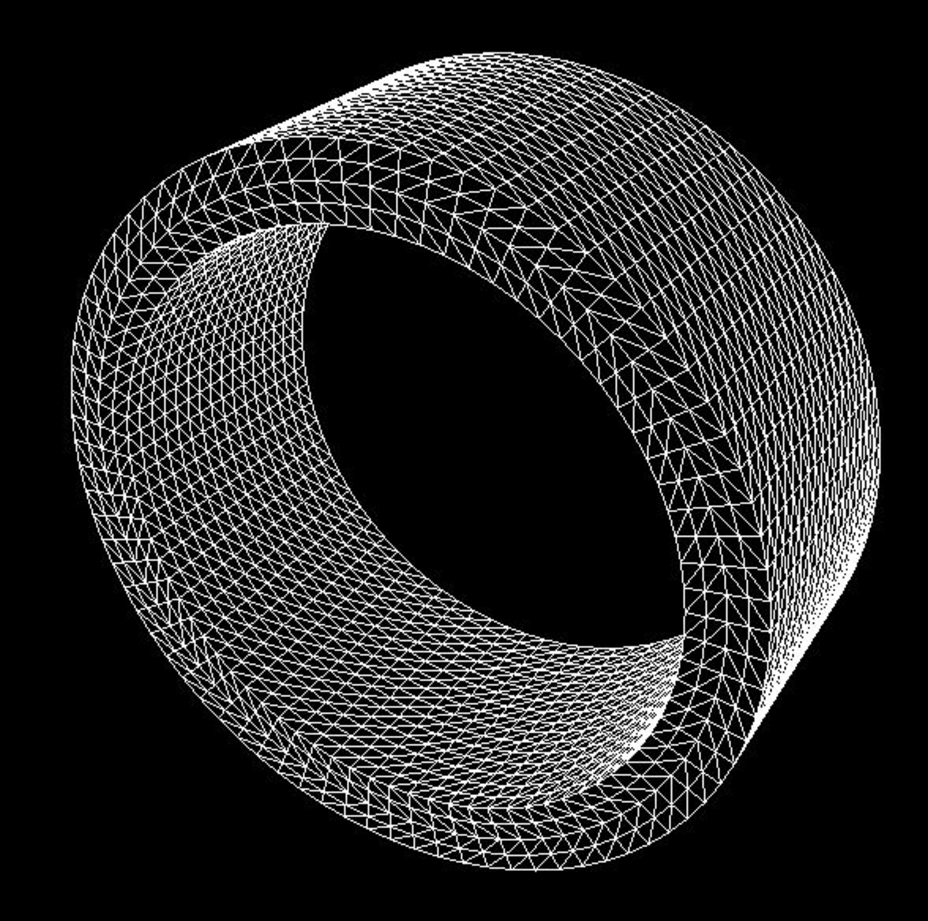
\includegraphics[width=0.35\textwidth]{4-5.pdf}
  \end{center}
  \caption{The metal tube.}
  \label{fig-dg-neighbor}
\end{figure}

And the figures below show deformed mesh for the 3-D metal tube:

\begin{figure}[H]
  \begin{center}
    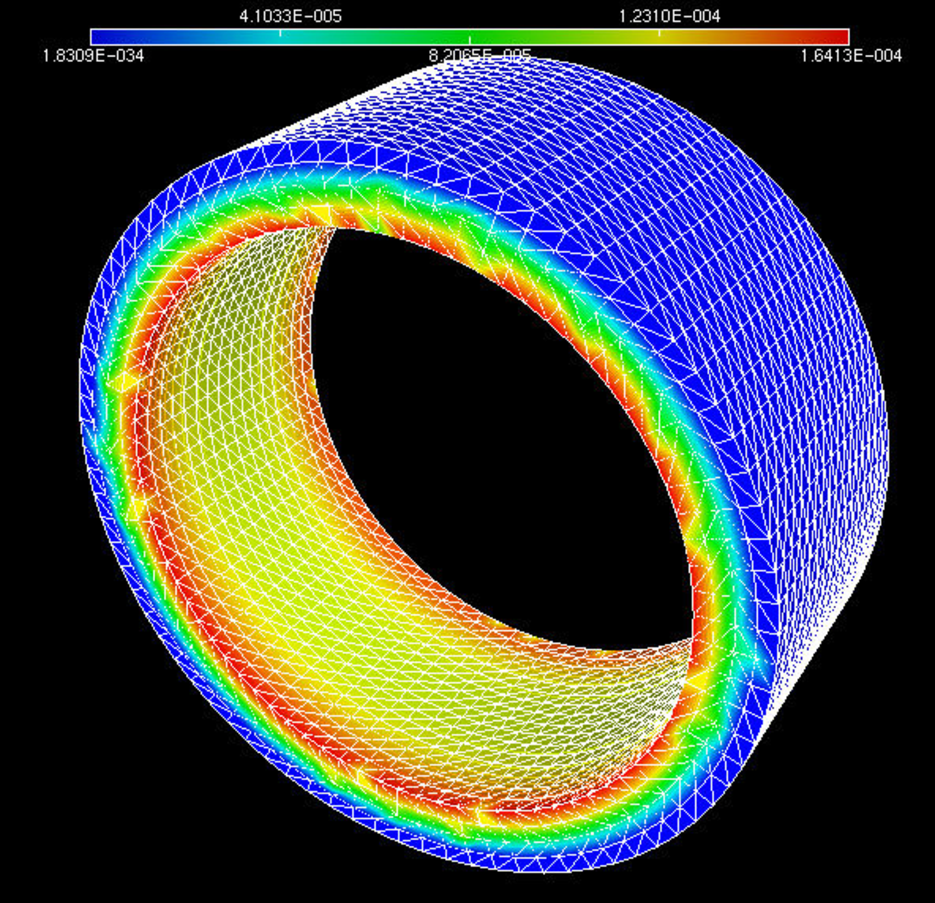
\includegraphics[width=0.35\textwidth]{4-5-1.pdf}
  \end{center}
  \caption{Deformed mesh for the 3-D metal tube (before).}
  \label{fig-dg-neighbor}
\end{figure}

\begin{figure}[H]
  \begin{center}
    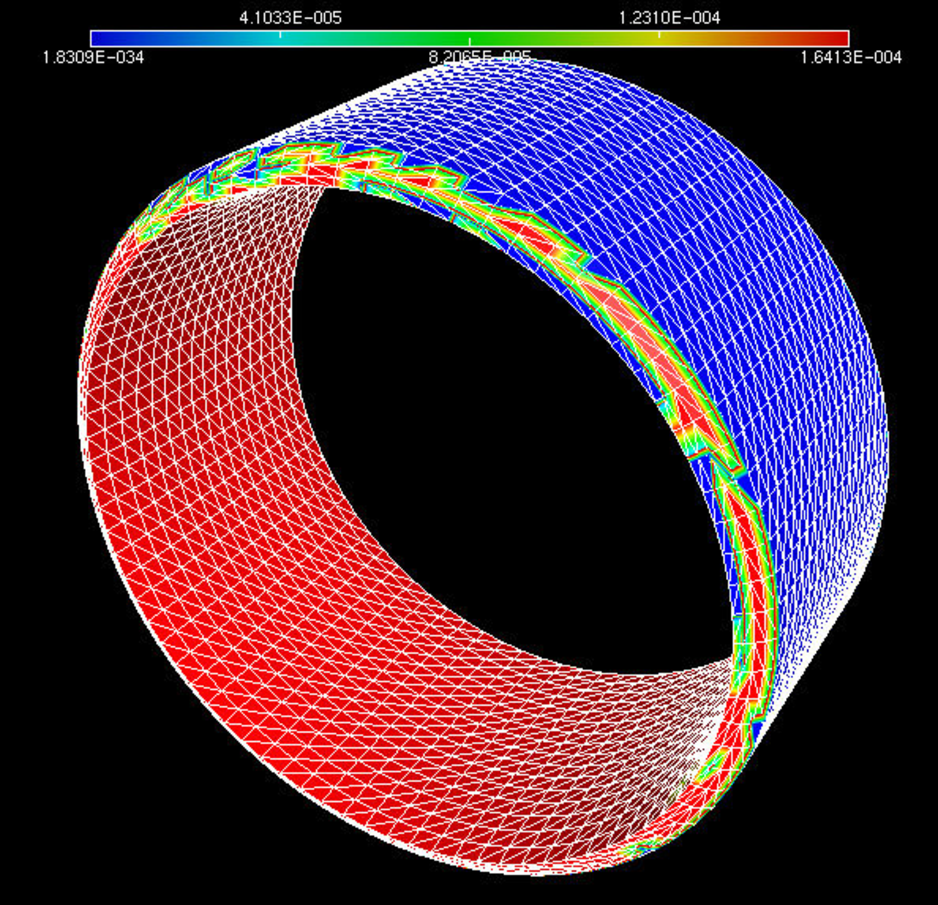
\includegraphics[width=0.35\textwidth]{4-5-2.pdf}
  \end{center}
  \caption{Deformed mesh for the 3-D metal tube (after).}
  \label{fig-dg-neighbor}
\end{figure}

\subsection{Fluid/Structures Coupled Problem}
In this example, we consider the Lam'e system of elasticity and the Stokes system for viscous fluids with velocity $u$ and pressure $p$:
$$-\Delta u + \nabla p = 0, \nabla .u = 0, \text{ in } \Omega, u = u_\Gamma \text{ on } \Gamma = \partial \Omega$$
where $u_\Gamma$ is the velocity of the boundaries. The force that the fluid applies to the boundaries is the normal stress:
$$h = (\nabla u + \nabla u^T)n - pn$$
The equations of elasticity are naturally written in variational form for the displacement vector $v(x)\in V$ as
$$\int_\Omega [2\mu \epsilon_{ij}(u)\epsilon_{ij}(v) + \lambda\epsilon_{ii}(u)\epsilon_{jj}(v)] = \int_\Omega g.v + \int_{\Gamma_N}h.v$$
where $g$ is the gravity force and h is the boundary stress.\\
\\
We consider the Lam'e system and the Stokes system are coupled by a common boundary on which the fluid stress creates a displacement of the boundary and hence changes the shape of the domain where the Stokes problem is integrated. The geometry is that of a vertical driven cavity with an elastic lid. The lid is a beam with weight so it will be deformed by its own weight and by the normal stress due to the fluid reaction. The cavity is the $10 * 10$ square and the lid is a rectangle of height $l = 2$. \\

\begin{figure}[H]
  \begin{center}
    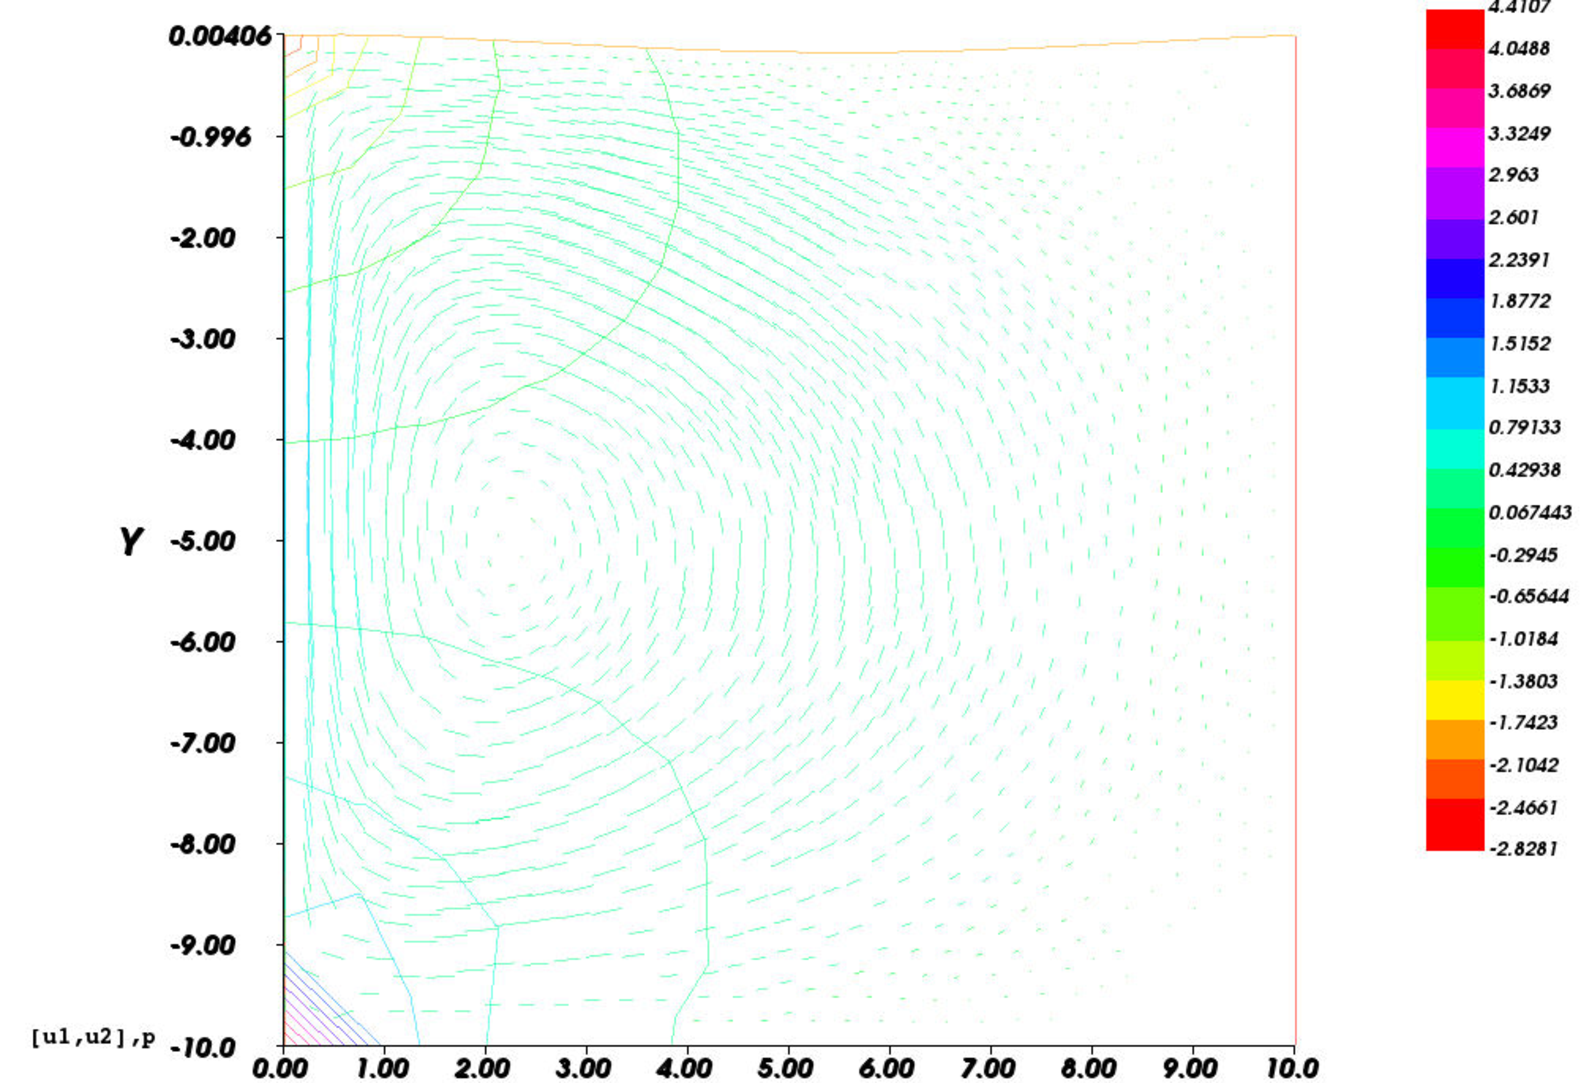
\includegraphics[width=0.5\textwidth]{4-6-1.pdf}
  \end{center}
  \caption{Fluid velocity and pressure in the fluid-structure interaction of a soft side and a driven cavity.}
  \label{fig-dg-neighbor}
\end{figure}

A beam sits on a box full of fluid rotating because the left vertical side has velocity one. The beam is bent by its own weight, but the pressure of the fluid modifies the bending. \\
The bending displacement of the beam is given as follows. \\

\begin{figure}[H]
  \begin{center}
    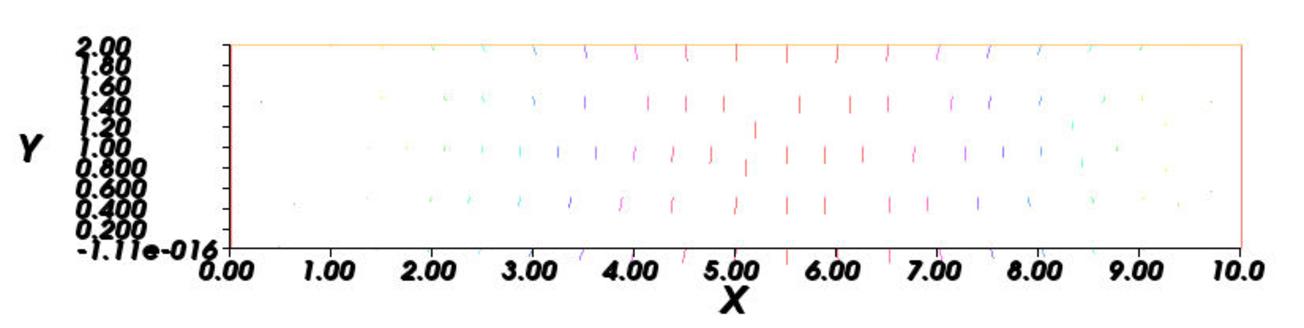
\includegraphics[width=0.5\textwidth]{4-6-2.pdf}
  \end{center}
  \caption{Displacement vector of the structure in the fluid-structure interaction of a soft side.}
  \label{fig-dg-neighbor}
\end{figure}

\begin{figure}[H]
  \begin{center}
    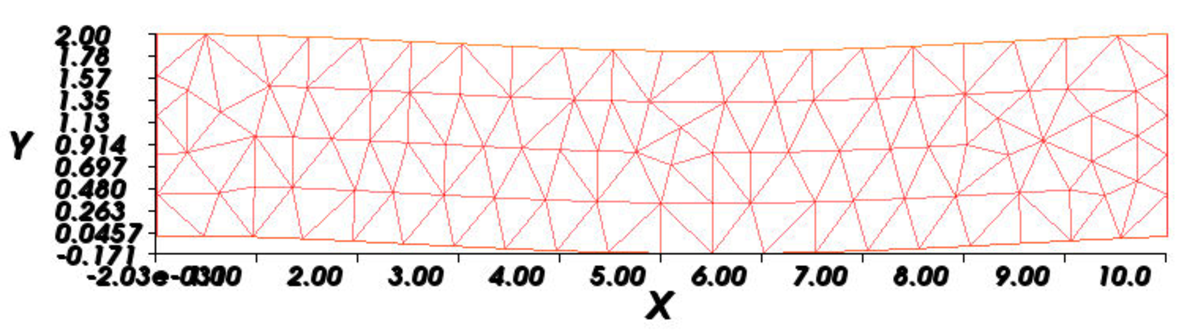
\includegraphics[width=0.5\textwidth]{4-6-3.pdf}
  \end{center}
  \caption{Displaced geometry in the fluid-structure interaction of a soft side.}
  \label{fig-dg-neighbor}
\end{figure}

%----------------------------------------------------------------------
\section{Conclusion and perspective}
\label{sec:conclusion}
We have presented the solver of linear elastic equation by continuous Galerkin finite element method which has the following advantages:
\begin{itemize}
  \item it allows for drastic shape deformation during the linear elasticity process.
  \item exhibit a nice application of this equation in Mechanical engineering.
  \item it can be extended to deal with other mechanical models, including nonlinear elasticity and design-dependent loads.
\end{itemize}
The efficiency and reliability of present work is numerical examples in 2D (Tractive force, Internal pressure) and 3D for linear elasticity problems. The program has been implemented in the FreeFem++ environment. It is noteworthy that the linear elastic problem becomes very interesting when it couple with Navier-Stokes equations, or a problem of shape optimization, e.g \cite{ABF97,AJT04}. For this reason, the source code are available online at \url{https://github.com/kangandroo/VIAMC2017}. 
\\
Any suggestions or contributions are welcome.

Regarding the perspectives, we would like to mention a few options:
\begin{itemize}
   \item Investigate the test cases in 3D with linear elasticity or non-linear elasticity system. 
   \item Couple with Navier-Stokes equations
   \item Combine the present scheme with a problem of shape-topology optimization \cite{AJT04}. This is an important feature when the elasticity solver is one of contribution for the future research in the problem of shape optimization in context of linear elasticity structure.
\end{itemize}
% --------------------------------------------------------------------
% biblio
% --------------------------------------------------------------------
\bibliographystyle{plain}
%\bibliography{biblio,florence-2016-autobib}
\bibliography{florence-2016-autobib}
\vfill
\end{multicols}
\end{document}
